\chapter{Daten}\label{ch:daten}

In diesem Kapitel wird zunächst die Wahl der Datenquelle erläutert, anschließend wird die konkrete Erzeugung des Ausgangsdatensatzes beschrieben.
Außerdem wird schrittweise die Verarbeitung des Ausgangsdatensatzes und die daraus resultierende Datenaggregation hin zu einem Evaluations- und Testdatensatzes aufgezeigt.
Der resultierende Datensatz stellt eines der zentralen Ergebnisse dieser Arbeit dar.

% ======================================================================================================================

% Hier wird beschrieben, welche Datenquelle ausgewählt wurde, warum sie ausgewählt wurde und welche Alternativen es gab.
\section{Wahl der Datenquelle}\label{sec:wahl-der-datenquelle}

Um einen Evaluations- und Testdaten zu erzeugen, muss zuerst eine geeignete Datenquelle identifiziert und gegen alternativen abgewogen werden.
Die Datenquelle wird anhand folgender Kriterien ausgewählt:
\begin{itemize}
    \item Verfügbarkeit -- die Datenquelle muss für die metaeffekt frei zugänglich sein.
    \item Realitätsnähe -- die Datenquelle muss reale Daten enthalten, künstliche Daten sollen weitgehend vermieden werden.
    \item Umfang -- der Datensatz soll einen für den Anwendungsfall ausreichenden Umfang haben.
    \item Reproduzierbarkeit und Erweiterbarkeit -- der Datensatz sollte durch einen reproduzierbaren Prozess erzeugt und idealerweise um weitere Quellen erweiterbar sein.
\end{itemize}

% TODO: Quelle einfügen
Das Github Repository des ScanCode-Toolkit beinhaltet einen Testdatensatz zur Erkennung von Copyrights.
Dieser Datensatz besteht aus mehreren tausend Dateien und ihren zugehörigen ScanCode-Ergebnissen.
Die Daten sind zum Teil in besondere Einzelfälle untergliedert, der Großteil der Daten ist jedoch unsortiert.
Da der Datensatz zum Testen der ScanCode Copyright Implementierung dient, beinhaltet er sowohl künstlich erzeugte Testfälle, als auch solche, die von Realdaten abgeleitet sind.

In Absprache mit dem Stakeholder wurde die Absicht, den Testdatensatz des ScanCode-Toolkit zu verwenden verworfen und stattdessen eine Datenquelle herangezogen, die einen möglichst heterogenen aber realen Datensatz beinhaltet.
Als Alternative Datenquelle wurde ein Alpine-Container gewählt.
Dieser Container wurde mithilfe des metaeffekt-Scanners analysiert und inventarisiert.
Das Scan-Ergebnis beinhaltet sämtliche im Container enthaltenen Quellcode-Dateien zusammen mit den entsprechenden MetaScan-Ergebnissen, sowie die durch den ScanCode-Service erzeugten Metadaten.
Der eindeutige Vorteil dieser Datenquelle besteht darin, dass es sich hierbei ausschließlich um Realdaten handelt, wie sie im Produktivbetrieb vorkommen.
Das Scan-Ergebnis ist außerdem um ein Vielfaches größer als der Testdatensatz des ScanCode-Toolkit.

% ======================================================================================================================

\section{Erzeugung des Ausgangsdatensatzes}\label{sec:erzeugung-datensatz}

Beim Scan des Alpine-Containers mithilfe des metaeffekt-Scanners laufen mehrere Schritte ab, die für die Aggregation eines Copyright-Datensatzes relevant sind.
Zunächst werden sämtliche Datenpakete entpackt und die resultierenden Quellcode-Dateien in eines oder mehrere Segmente unterteilt.
Die resultierenden Segmente werden normalisiert und auf diese normalisierten Segmente werden Scan-Prozesse, wie der ScanCode-Service, angewandt.

Das vom ScanCode-Service erzeugte Ergebnis enthält die ermittelten Copyright-Informationen für ein normalisiertes Segment.
Die Normalisierung umfasst unter anderem das Entfernen mehrfacher Leerzeichen sowie von Zeilenumbrüchen.
Die \nameref{subsec:cep-01} besagt, dass Copyright-Statements nicht verändert werden dürfen.
Da die Normalisierung und Segmentierung den originalen Zustand der Datei verändern, können sie nicht für den Datensatz herangezogen werden.
Stattdessen werden die in den Segmenten referenzierten Originaldateien ermittelt und für jede Datei die Scan-Ergebnisse aller ihrer Segmente zusammengeführt.

% TODO: Eventuell hier kurz darauf eingehen, dass der SHA-1 Hash gewählt wurde, um kollisionen zu vermeiden und von originalen Dateinamen zu abstrahieren. Wahrscheinlichkeit für Kollision nennen.
Um Namenskonflikte zu vermeiden, wurde anschließend für jede Originaldatei der SHA-1 Hash berechnet und zusammen mit dem Dateityp zur Benennung der Datei verwendet.
Da die Verzeichnisstruktur der Originaldateien nicht relevant ist, werden alle Dateien in einem flachen Verzeichnis gespeichert, dies vereinfacht die anschließende Verarbeitung zusätzlich.
Der resultierende Ausgangsdatensatz umfasst etwa \num{467000} Originaldateien und ihre Scan-Ergebnisse.

% ======================================================================================================================

\section{Analyse des Datensatzes und Kategorisierung der Daten}\label{sec:analyse-datensatz}

Der erzeugte Datensatz kann in seiner extrahierten Form noch nicht zur Evaluation und Test verwendet werden, da die Scan-Ergebnisse nicht auf den Originaldateien, sondern auf ihren normalisierten Segmenten beruhen.
Um diese Problematik zu adressieren, muss ein Prozess bestimmt werden, der bereits korrekte Daten ermittelt und fehlerhafte Daten, sofern möglich, korrigiert.
Korrekt bedeutet in diesem Kontext, dass die extrahierten Daten der Policy entsprechen.
Dieser Prozess wird nachfolgend schrittweise beschrieben:

\textbf{Schritt 1 -- Unterteilung nach ScanCode-Ergebnissen.}
Der Datensatz wurde in zwei Kategorien unterteilt: Dateien, für die ScanCode \enquote{copyrights}, \enquote{holders} bzw. \enquote{authors} ermitteln konnte, und solche, die keine der genannten Informationen enthalten.
Etwa zwei Drittel des Datensatzes gehören zur letzteren Kategorie.
Die Daten ohne ScanCode-Ergebnis sind allerdings dennoch relevant, da es sich hierbei um False-Negatives des ScanCode-Toolkit handeln kann, die zur Verbesserung der Extraktion unbedingt ermittelt werden müssen.

\textbf{Schritt 2 -- Entfernung von Duplikaten.}
Zunächst wurden Duplikate aus dem Datensatz mit ScanCode-Ergebnissen entfernt.
Hierzu wurden Daten mit demselben SHA-1 Hash ermittelt und alle Duplikate eliminiert.
Diese Filterung reduzierte den Datensatz um etwa 8\,\%.

\textbf{Schritt 3 -- Trennung von Einträgen ohne Copyrights.}
Der von Duplikaten bereinigte Datensatz wurde danach unterteilt, ob das ScanCode-Ergebnis ausschließlich \enquote{authors} enthält.
% TODO: Kategorie von contains no copyrigths zu contains only authors umbenennen.
Diese Kategorie von Daten ohne Copyrights (\enquote{contains only authors}) umfasst ca.\ 11\,000 Dateien und dient dazu, die Extraktion auf False-Positives beim Erkennen der \enquote{copyrights} zu analysieren.
Außerdem kann dieser Datensatz genutzt werden, das Extrahieren von Autoren gezielt und isoliert zu untersuchen.

\textbf{Schritt 4 -- Abgleich mit Originaldateien (\enquote{exact matches}).}
Die extrahierten Copyright-Statements der ScanCode-Ergebnisse wurden in den entsprechenden Originaldateien gesucht.
Wenn eine Originaldatei jedes der extrahierten Statements exakt enthält, wurde diese Datei und ihr extrahiertes Ergebnis den \enquote{exact matches} zugeordnet.
Das exakte Vorkommen des extrahierten Statements in der Originaldatei erfüllt die Bedingung einer Extraktion \enquote{as-is} gemäß \nameref{subsec:cep-01}.
ScanCode-Ergebnisse, die einen \enquote{exact match} aufweisen und keine Blöcke von Copyrights beinhalten (siehe \nameref{subsec:cep-03}), sind demnach ohne weitere Verarbeitung in Hinsicht auf ihre \enquote{copyrights} Policy-konform.
Blöcke von Copyright-Statements können zwar für jedes extrahierte Statement einen \enquote{exact match} aufweisen, verstoßen aber durch ihre ScanCode bedingte Aufteilung gegen die \nameref{subsec:cep-03}.
Eine korrekte Extraktion der \enquote{holder} und \enquote{authors} erfordert komplexere Mechanismen und wird im Laufe der Arbeit hauptsächlich durch manuelle Überprüfung gewährleistet.
Da die Priorisierung der Extraktion bei einer korrekten Extraktion der \enquote{copyrights} liegt, werden die möglicherweise fehlerhaft extrahierten Urheber und Autoren als verkraftbares Übel hingenommen.

\textbf{Schritt 5 -- Analyse und Rekonstruktion der \enquote{no exact matches}}
Die ScanCode-Ergebnisse ohne \enquote{exact match} umfassen ca.\ zwei Drittel des Datensatzes.
Die Analyse dieser Ergebnisse zeigte, dass ScanCode unter anderem die Groß- und Kleinschreibung der Statements normalisiert.
Ein Beispiel hierfür ist die konsequente Ersetzung der \enquote{(C)} Markierung durch \enquote{(c)}.
Um diese Fälle zu identifizieren, wurden alle Originaldateien und ihre ScanCode-Ergebnisse in Kleinbuchstaben umgewandelt und anschließend überprüft, ob für jedes extrahierte Statement ein \enquote{exact match} vorliegt.
Wenn ein solcher Match vorlag, konnte geschlussfolgert werden, dass die einzige Differenz zwischen Originaldatei und Extrakt die Groß- bzw.\ Kleinschreibung war.
Dieser Teil des Datensatzes wurde der Kategorie \enquote{exact matches without case} zugeordnet und die enthaltenen Fälle wurden anschließend zu \enquote{exact matches} aufgewertet.
Die Rekonstruktion der Original-Statements erfolgte, indem das extrahierte Statement in der Originaldatei gesucht und anschließend das Original-Statement im Ergebnis ersetzt wurde.
Auf diese Weise konnten ca.\ \num{57000} Dateien den \enquote{exact matches} hinzugefügt werden.

\textbf{Schritt 6 -- Rekonstruktion der Formatierung.}
Da sowohl durch das ScanCode-Toolkit als auch durch die metaeffekt Prozesse Normalisierungen stattfinden, gehen Formatierungen with Zeilenumbrüche und Tabulatoren bzw.\ mehrfache Leerzeichen verloren.
Um die \nameref{subsec:cep-06} zu erfüllen, muss die Formatierung im extrahierten Copyright-Statement erhalten bleiben.
Die durch Normalisierung betroffenen Statements wurden dadurch identifiziert, dass aus den Originaldateien und ScanScode-Ergebnissen jegliche Formatierungen, also Leerzeichen, Zeilenumbrüche und Tabulatoren entfernt wurden.
Anschließend wurde überprüft, ob für jedes Statement einer Datei ein \enquote{exact match} vorliegt.
Die Rekonstruktion dieser \enquote{exact matches without format} erfordert, dass das Statement in der Originaldatei gefunden und anschließend in das ScanCode-Ergebnis kopiert wird.
Da die Statements durch ihre Formatierung nicht eindeutig dem Ergebnis zuweisbar sind, wurde die Levenstein-Distanz zwischen den extrahierten Statements und jedem Substring der Originaldatei berechnet und der Substring gewählt, welcher die geringste Distanz zum Statement ergab.
Anschließend wurden alle Zeichen zwischen dem ersten und letzten Index des Substring aus der Originaldatei in das ScanCode-Ergebnis übertragen.
Durch diese Methode konnten ca.\ \num{6000} \enquote{exact matches without case} rekonstruiert werden.
Die Statements erfordern dennoch Teils manuelle Arbeit, da bei mehrzeiligen Statements die in Kommentarsyntax eingebettet sind, nun auch die entspreche Kommentarsyntax in die Metadaten übertagen wurde.
Die Kategorie \enquote{exact match without format and case} enthält solche Fälle, die sowohl abweichende Formatierung als auch abweichende Groß- und Kleinschreibung im ScanCode-Ergebnis enthalten.
Die Fälle dieser Kategorie wurden dadurch ermittelt, dass zunächst jegliche Formatierung und dann jede Großschreibung in den Originaldateien und den ScanCode-Ergebnissen entfernt wurde, anschließend wurde auch \enquote{exact matches} geprüft.
Von den ursprünglichen rund \num{94000} \enquote{no exact matches} gehören nach den vorherigen Schritten noch ca.\ \num{27000} Dateien der Kategorie \enquote{other reasons} an.
Diese Kategorie erfordert weitere Untersuchungen und eventuell manuelle Aufbereitung.

\textbf{Schritt 7 -- Identifizierung von\enquote{multiple copyrights}.}
Die \enquote{exact matches} wurden danach unterteilt, ob das entsprechende ScanCode-Ergebnis mehrere oder nur ein einzelnes Statement beinhalten.
Die Datei, welche mehrere Statements beinhalten wurde der Kategorie \enquote{multiple copyrights} zugeordnet und anschließend erneut unterteilt, je nachdem ob sie \enquote{authors} enthalten oder nicht.
Die Absicht bei der Unterteilung nach \enquote{multiple copyrights} und die anschließende Unterteilung nach \enquote{authors} soll dazu dienen, dass bei späteren Erstellen von Benchmark bzw.\ Evaluationsdatensätzen möglichst viele Formen von Copyrights in vergleichbarer Anzahl vorhanden sind.
Da die meisten Copyright-Statements im Datensatz einzelne Copyrights ohne Autoren sind, ist es wichtig, keinen Bias aufgrund dieser Datenlage zu erzeugen.

\textbf{Schritt 8 -- Identifizierung von \enquote{single copyrights}.}
Analog zu den \enquote{multiple copyrights} wurden die \enquote{single copyrights} identifiziert und nach dem Vorkommen von \enquote{authors} unterteilt.
Die resultierenden Kategorien \enquote{single copyrights with authors} und \enquote{single copyrights without auhtors} sind die zwei größten Unterkategorien des Datensatzes mit ca.\ \num{20000} Dateien ohne und ca.\ \num{70000} Dateien mit \enquote{authors}.

\begin{figure}[ht]
    \centering
    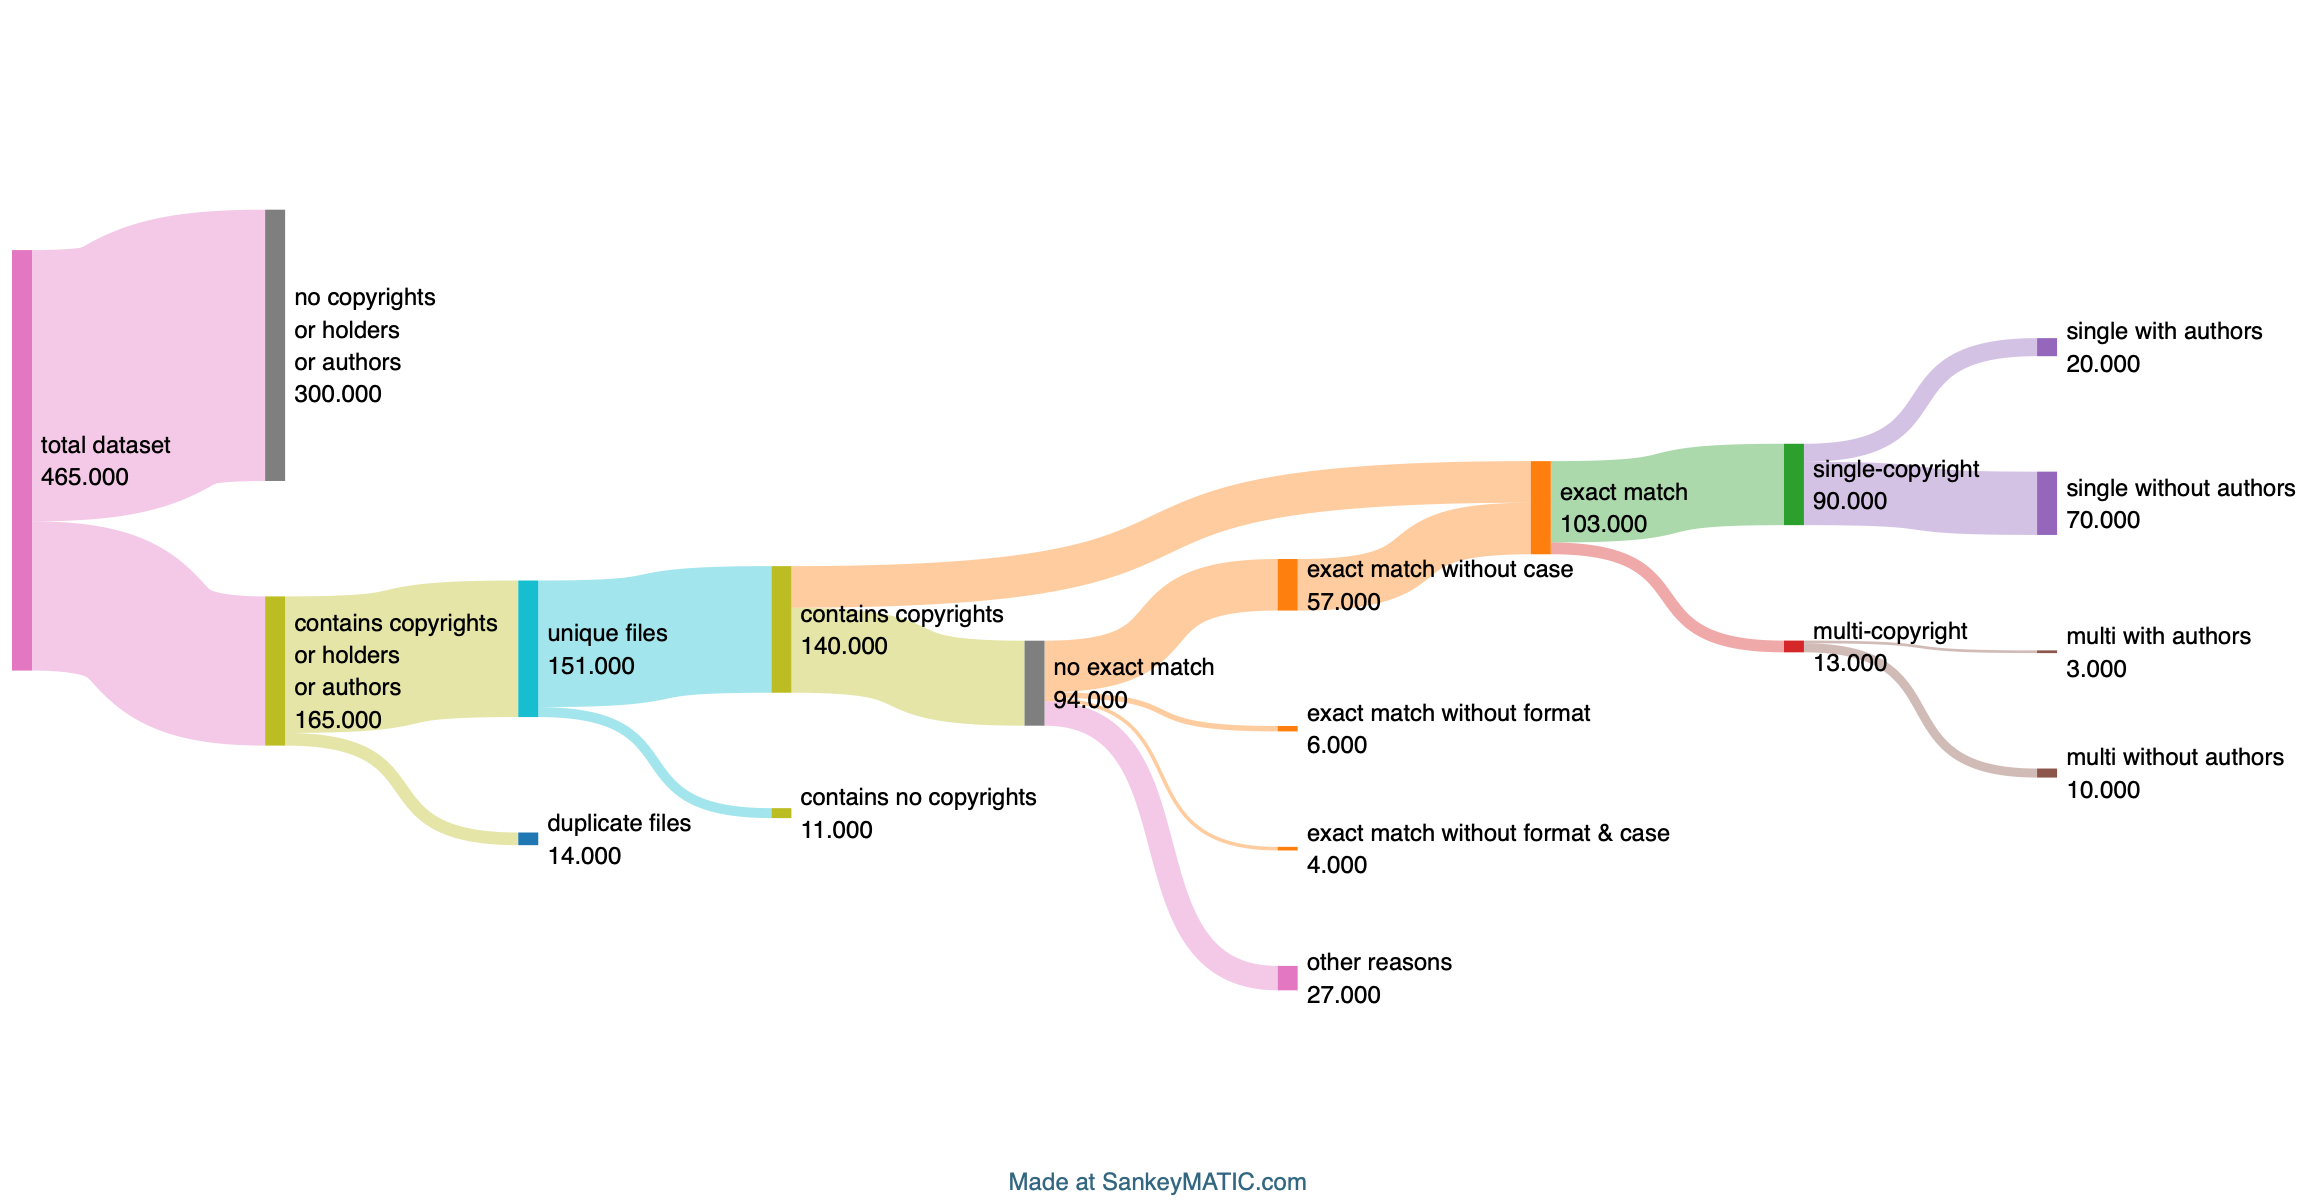
\includegraphics[width=16cm]{daten/sanky-daten}
    \caption{Sanky-Diagramm der verschiedenen Kategorien von ScanCode-Ergebnissen bei der Datenaggregation. Das Diagramm veranschaulicht die schrittweise Bildung von Datenkategorien sowie die Anzahl der Quellcode-Dateien pro Zwischenschritt.}
    \label{fig:sanky-daten}
\end{figure}
Das Resultat der Datenaggregation sind neun Kategorien von Dateien in Hinsicht auf ihr ScanCode-Ergebnis, welche unterschiedliche Qualitätsstufen in Hinsicht auf die Policy und auf den Aufwand in ihrer Nachbereitung aufweisen.
Die \autoref{fig:sanky-daten} veranschaulicht die schrittweise Verarbeitung und Kategorisierung der Daten.
Besonders bei der Abbildung hervorzuheben ist einerseits die Zusammenführung der \enquote{exact matches} und der rekonstruierten \enquote{exact matches without case}, welche den größten Anteil des Datensatzes ausmachen.
Außerdem kann der geneigte Leser anhand der Abbildung erkennen, in welchem Größenverhältnis die verschiedenen Kategorien zueinander stehen bzw.\ welche Kategorien den geringsten Teil des Datensatzes abdecken.
Die aggregierten Kategorien dienen in den folgenden Untersuchungen dazu, möglichst unterschiedliche Testdaten zu wählen und dabei möglichst viele Gestalten von Copyrights zu prüfen.

% ======================================================================================================================

% Hier soll darauf eingegangen werden, welche Probleme und Herausforderungen der Datensatz mit sich gebracht hat, einige
% davon sind die Größe (170GB), die Encodings, Binary-Dateien und die geringe Qualität der Scancode extraktion im "authors" Feld.
\section{Herausforderungen bei der Datenaggregation}\label{sec:herausforderungen-datenaggregation}

% ======================================================================================================================

% Hier soll darauf eingegangen werden, welche Probleme/Qualitätseinbußen der Datensatz aufzuweisen hat, darüber hinaus soll erläutert werden, warum der Datensatz gut ist
% Der Datensatz ist nicht gut weil es keinen besseren gibt -> vielleicht ist ein besserer nur nicht bekannt, stattdessen
% ist der Datensatz mit dem aktuellen Industriestandard (ScanCode) erzeugt worden und wurde nach der von uns erstellten Policy verbessert und validiert
\section{Qualität der Daten}\label{sec:qualitaet-der-daten}


